
\documentclass{article}

\usepackage{pttyr_descriptions}


\begin{document}

\setlist{nolistsep}
\nointerlineskip
\par\noindent
\setlength{\parindent}{0pt}


\section*{Shape}
\subsection*{\texttt{torch.Tensor.size}, \texttt{torch.Tensor.stride}}
\prepost{a.size() or a.stride()}{
  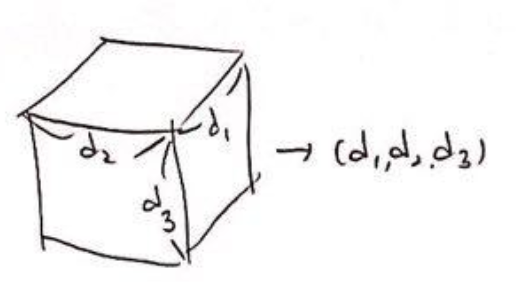
\includegraphics[height=8em]{resources/size1.png}
}{
  \begin{itemizec}
    \item $|\mtt{a}| = (d_1, d_2, \dots, d_k)$
  \end{itemizec}
}{
  \begin{itemizec}
    \item $(d_1, d_2, \dots, d_k)$를 튜플로 반환
  \end{itemizec}
}
\begin{align*}
  \forall \mtt{ft} \in \{ \mtt{size}, \mtt{stride}, \},\bigspace
  \frac
  {
    \begin{array}{l}
      \sigma \vdash E \Rar e, c
    \end{array}
  }
  {
    \sigma \vdash E.\op{ft}{} \Rar shapeToTuple(e), c
  }
\end{align*}

\prepost{a.size(n)}{
  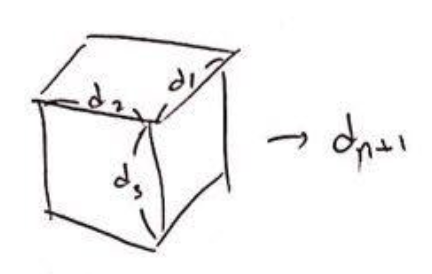
\includegraphics[height=8em]{resources/size2.png}
}{
  \begin{itemizec}
    \item $|\mtt{a}| = (d_1, d_2, \dots, d_k)$
    \item $0 \leq n < k$
  \end{itemizec}
}{
  \begin{itemizec}
    \item $d_{n+1}$을 숫자(int)로 반환
    \item $n$에 $-1$이 들어갈 수도 있음
  \end{itemizec}
}
\begin{align*}
  \forall \mtt{ft} \in \{ \mtt{size}, \mtt{stride}, \},\bigspace
  \frac
  {
    \begin{array}{l}
      \sigma \vdash E \Rar e, c \\
      k = \op{rank}{e} \\
      c' = \{ (k \geq 1) \land (0 \leq n < k) \}
    \end{array}
  }
  {
    \sigma \vdash E.\op{ft}{n} \Rar e\ind{n+1}, c \cup c'
  }
\end{align*}

\subsection*{\texttt{torch.Tensor.shape}}
\prepost{a.shape}{
  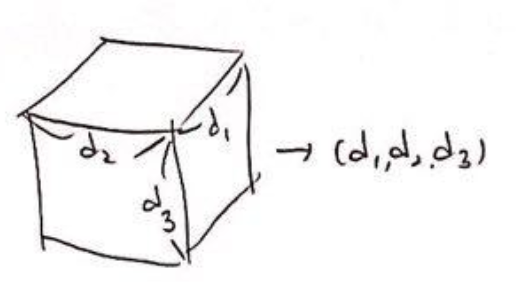
\includegraphics[height=8em]{resources/size1.png}
}{
  \begin{itemizec}
    \item $|\mtt{a}| = (d_1, d_2, \dots, d_k)$
  \end{itemizec}
}{
  \begin{itemizec}
    \item $(d_1, d_2, \dots, d_k)$를 튜플로 반환
  \end{itemizec}
}
\begin{align*}
  \frac
  {
    \begin{array}{l}
      \sigma \vdash E \Rar e, c
    \end{array}
  }
  {
    \sigma \vdash E.\mtt{shape} \Rar shapeToTuple(e), c
  }
\end{align*}

\section*{Tensor Declarations}
\subsection*{\texttt{torch.tensor}}
\onlyc{torch.tensor(x)}{}{\texttt{numpy}나 파이썬 리스트로 선언된 객체를
\texttt{torch}에서 호환가능한 형태로 바꾸는 함수}
\begin{align*}
  \frac
  {
    \sigma \vdash {E} \Rar e, c
  }
  {
    \sigma \vdash \op{tensor}{E} \Rar e, c
  }
\end{align*}

\subsection*{\texttt{torch.range}, \texttt{torch.arange}}
\prepostc{torch.range(start=0, end, step=1, out=None, ...), torch.arange(...)}{
  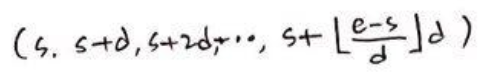
\includegraphics[width=\linewidth]{resources/range.png}
}{
  \begin{itemizec}
    \item $step \neq 0$
    \item $(end - start)/step > 0$
  \end{itemizec}
}{
  \begin{itemizec}
    \item $|y| = (1 + \lfloor (end - start)/step \rfloor)$
  \end{itemizec}
}{
  \begin{itemizec}
      \item $(start, start+step, start+2\cdot step, \dots)$를 반환
      \item $out$-텐서 인자가 있는 함수
      \item \texttt{torch.arange}도 똑같은 방식으로 작동함
    \end{itemizec}
}
\begin{align*}
  \forall \mtt{ft} \in \{ \mtt{range}, \mtt{arange} \},\bigspace
  \frac
  {
    \begin{array}{l}
      c = \{(d \neq 0) \land ((e-s)/d > 0)\}
    \end{array}
  }
  {
    \sigma \vdash \op{ft}{s, e, d, out=None, ...} \Rar
      (1+\lfloor (e-s)/d \rfloor), c
  }
  \tag*{Default: $s = 0, d = 1$}
\end{align*}
 
\subsection*{\texttt{torch.linspace}}
\prepostc{torch.linspace(start, end, steps=100, out=None, ...)}{
  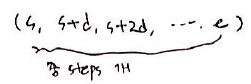
\includegraphics[height=6em]{resources/linspace.png}
}{
  \begin{itemizec}
    \item $steps \geq 0$
  \end{itemizec}
}{
  \begin{itemizec}
    \item $|y| = (steps)$
  \end{itemizec}
}{
  \begin{itemizec}
    \item $(start, start+d, start+2d, \dots, end)$인데 원소가 $steps$개인 텐서 반환
    \item $out$-텐서 인자가 있는 함수
  \end{itemizec}
}
\begin{align*}
  \frac
  {
    \begin{array}{l}
      c = \{(steps \geq 0)\}
    \end{array}
  }
  {
    \sigma \vdash \op{linspace}{s, e, steps=100, out=None, ...} \Rar (steps), c
  }
\end{align*}

\subsection*{\texttt{torch.zeros}, \texttt{torch.empty}, \texttt{torch.rand},
\texttt{torch.randn}}
\prepostc{torch.zeros(t1, t2, ..., tl, out=None, ...) or .empty, .rand,
.randn}{}{}{
  \begin{itemizec}
    \item $|y| = (t_1, t_2, \dots, t_l)$
  \end{itemizec}
}{
  \begin{itemizec}
    \item 입력받은 형태대로 $0$, uninitialized, uniformly random, gaussian
    random 텐서를 반환
    \item $(t_1, t_2, \dots, t_l)$ 입력이 하나의 튜플로 들어오는 경우도 있음
    \item $out$-텐서 인자가 있는 함수
  \end{itemizec}
}
\begin{align*}
  \forall \mtt{ft} \in \{\mtt{zeros}, \mtt{empty}, \mtt{rand}, \mtt{randn}\},
  \bigspace
  \frac
  {
  }
  {
    \sigma \vdash \op{ft}{t_1, t_2, \dots, t_l, out=None} \Rar (t_1, t_2, \dots, t_l),
      \emptyset
  }
\end{align*}
\begin{align*}
  \forall \mtt{ft} \in \{\mtt{zeros}, \mtt{empty}, \mtt{rand}, \mtt{randn}\},
  \bigspace
  \frac
  {
  }
  {
    \sigma \vdash \op{ft}{(t_1, t_2, \dots, t_l), out=None} \Rar (t_1, t_2, \dots, t_l),
      \emptyset
  }
\end{align*}

\subsection*{\texttt{torch.randint}}
\prepostc{torch.randint(low=0, high, shape, ..., out=None, ...)}{}{
  \begin{itemizec}
    \item $low < high$
    \item $shape$가 well-defined인 텐서 shape. (스칼라 타입은 X)
  \end{itemizec}
}{
  \begin{itemizec}
    \item $|y| = shape$
  \end{itemizec}
}{
  \begin{itemizec}
    \item $low$부터 $high-1$까지 랜덤한 정수 할당
    \item $out$-텐서가 있는 함수
  \end{itemizec}
}
\begin{align*}
  \frac
  {
  }
  {
    \sigma \vdash \op{randint}{low=0, high, (t_1, t_2, \dots, t_l), ...,
    out=None, ... } \Rar (t_1,
    t_2, \dots, t_l), \{(low < high)\}
  }
\end{align*}

\subsection*{\texttt{torch.randperm}}
\prepostc{torch.randperm(n, out=None, ...)}{}{
  \begin{itemizec}
    \item $n \geq 0$
  \end{itemizec}
}{
  \begin{itemizec}
    \item $|y| = (n)$
  \end{itemizec}
}{
  \begin{itemizec}
    \item $out$-텐서가 있는 함수
  \end{itemizec}
}
\begin{align*}
  \frac
  {
  }
  {
    \sigma \vdash \op{randperm}{n, out=None, ... } \Rar (n), \{(n \geq 0)\}
  }
\end{align*}

\subsection*{\texttt{torch.full}}
\prepostc{torch.full((t1, t2, ..., tl), fill\_value, out=None, ...)}{}{}{
  \begin{itemizec}
    \item $|y| = (t_1, t_2, \dots, t_l)$
  \end{itemizec}
}{
  \begin{itemizec}
    \item 모든 원소가 $fill\_value$로 채워진 텐서 반환
    \item \texttt{empty}랑 비슷해보이는데, size인자를 항상 튜플로만 받음
    \item $out$-텐서가 있는 함수
  \end{itemizec}
}
\begin{align*}
  \frac
  {
  }
  {
    \sigma \vdash \op{full}{(t_1, t_2, \dots, t_l), fill\_value, out=None} \Rar (t_1, t_2, \dots, t_l),
      \emptyset
  }
\end{align*}
 
\subsection*{\texttt{torch.normal}}
\prepostc{torch.normal(mean, std, (t1, t2, ..., tl), out=None}{}{
  \begin{itemizec}
    \item $std > 0$
  \end{itemizec}
}{
  \begin{itemizec}
    \item $|y| = (t_1, t_2, \dots, t_l)$
  \end{itemizec}
}{
  \begin{itemizec}
    \item \texttt{empty}랑 비슷해보이는데, size인자를 항상 튜플로만 받음
    \item $out$-텐서가 있는 함수
  \end{itemizec}
}
\begin{align*}
  \frac
  {
  }
  {
    \sigma \vdash \op{normal}{mean, std, (t_1, t_2, \dots, t_l), out=None} \Rar (t_1, t_2, \dots, t_l),
      \{ (std > 0) \}
  }
\end{align*}

\subsection*{\texttt{torch.Tensor.new\_empty}}
\prepostc{x.new\_empty((t1, t2, ..., tl), ...)}{}{}{
  \begin{itemizec}
    \item $|y| = (t_1, t_2, \dots, t_l)$
  \end{itemizec}
}{
  \begin{itemizec}
    \item \texttt{empty}랑 비슷해보이는데, \texttt{Tensor} 클래스에서만 사용
    가능하고, $out$인자도 없으며, size인자를 항상 튜플로만 받음
    \item 텐서 \texttt{x}의 shape도 똑같이 변함
  \end{itemizec}
}
\begin{align*}
  \frac
  {
  }
  {
    \sigma \vdash x.\op{new\_empty}{(t_1, t_2, \dots, t_l), ...} \Rar (t_1, t_2, \dots, t_l),
      \emptyset
  }
  \\
  \text{$x$의 shape도 똑같이 $(t_1, t_2, \dots, t_l)$로 변함}
\end{align*}

\subsection*{\texttt{torch.Tensor.new\_full}}
\prepostc{x.new\_full((t1, t2, ..., tl), fill\_value, ...)}{}{}{
  \begin{itemizec}
    \item $|y| = (t_1, t_2, \dots, t_l)$
  \end{itemizec}
}{
  \begin{itemizec}
    \item \texttt{new\_empty}랑 비슷해보이는데, \texttt{fill\_value} 인자가
    추가적으로 있음
    \item 텐서 \texttt{x}의 shape도 똑같이 변함
  \end{itemizec}
}
\begin{align*}
  \frac
  {
  }
  {
    \sigma \vdash x.\op{new\_full}{(t_1, t_2, \dots, t_l), fill\_value...} \Rar (t_1, t_2, \dots, t_l),
      \emptyset
  }
  \\
  \text{$x$의 shape도 똑같이 $(t_1, t_2, \dots, t_l)$로 변함}
\end{align*}
 
\subsection*{\texttt{torch.Tensor.clone}}
\prepost{x.clone(...)}{}{}{
  \begin{itemizec}
    \item $|y| = |x|$
  \end{itemizec}
}
\begin{align*}
  \frac
  {
    \sigma \vdash E \Rar e, c
  }
  {
    \sigma \vdash E.\op{clone}{...} \Rar e, c
  }
\end{align*}

\subsection*{\texttt{torch.zeros\_like}, \texttt{torch.empty\_like},
\texttt{torch.rand\_like}, \texttt{torch.randn\_like}}
\prepostc{torch.zeros\_like(input, ...) or .empty\_like, .rand\_like,
.randn\_like}{}{}{
  \begin{itemizec}
    \item $|y| = |input|$
  \end{itemizec}
}{
  \begin{itemizec}
    \item 입력받은 텐서와 shape이 같은 $0$, uninitialized, uniformly random,
    gaussian random 텐서를 반환
    \item $out$-텐서 인자가 없음!
  \end{itemizec}
}
\begin{align*}
  \forall \mtt{ft} \in \{\mtt{zeros\_like}, \mtt{empty\_like}, \mtt{rand\_like}, \mtt{randn\_like}\},
  \bigspace
  \frac
  {
    \sigma \vdash E \Rar e, c
  }
  {
    \sigma \vdash \op{ft}{E, ...} \Rar e, c
  }
\end{align*}

\subsection*{\texttt{torch.full\_like}}
\prepostc{torch.full\_like(input, fill\_value, out=None, ...)}{}{}{
  \begin{itemizec}
    \item $|y| = |input|$
  \end{itemizec}
}{
  \begin{itemizec}
    \item 입력받은 텐서와 shape이 같은 $fill\_value$로 가득찬 텐서 반환
    \item 희한하게 이건 $out$-텐서 인자가 있음..
  \end{itemizec}
}
\begin{align*}
  \frac
  {
    \sigma \vdash E \Rar e, c
  }
  {
    \sigma \vdash \op{full\_like}{E, fill\_value, out=None...} \Rar e, c
  }
\end{align*}

\subsection*{\texttt{torch.scalar\_tensor}}
\prepostc{torch.scalar\_tensor(scalar, ...)}{
  
\includegraphics[height=3em]{resources/scalar_tensor.png}
}{}{
  \begin{itemizec}
    \item $|y| = ()$
  \end{itemizec}
}{
  \begin{itemizec}
    \item $scalar$ 값 하나만 가지는 $\mtt{rank}$-$0$ 텐서 반환
  \end{itemizec}
}
\begin{align*}
  \frac
  {
  }
  {
    \sigma \vdash \op{scalar\_tensor}{scalar, ...} \Rar (), \emptyset
  }
\end{align*}
 
\subsection*{\texttt{torch.eye}}
\prepostc{torch.eye(n, m=None, out=None, ...)}{
  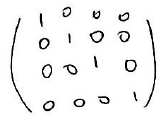
\includegraphics[height=8em]{resources/eye.png}
}{
  \begin{itemizec}
    \item $n \geq 0$
    \item $m = None$ or $m \geq 0$
  \end{itemizec}
}{
  \begin{itemizec}
    \item $|y| = \left\{
      \begin{array}{ll}
        (n, n) & \text{if $m$ is $None$} \\
        (n, m) & \text{otherwise}
      \end{array}
      \right.
    $
  \end{itemizec}
}{
  \begin{itemizec}
    \item 곱셈의 항등원 $I_n$를 리턴
    \item $out$ 인자가 있는 함수
  \end{itemizec}
}
\begin{align*}
  \frac
  {
    \begin{array}{l}
      e = \ifs{m = None}{(n, n)}{(n, m)} \\
      c = \{ (n \geq 0) \land (m = None \lor m \geq 0) \}
    \end{array}
  }
  {
    \sigma \vdash \op{eye}{n, m, out=None, ...} \Rar e, c
  }
\end{align*}

\section*{Same Shape, Elementwise Operators}
All these builtin functions \texttt{torch.*} are used with
\texttt{torch.ft(input, out=None)} that output the same shapes of the
\texttt{input}s.
\begin{itemize}
  \item $\mtt{round}, \mtt{floor}, \mtt{ceil}$
  \item $\mtt{exp}, \mtt{log}, \mtt{log10}, \mtt{log2}, \mtt{log1p},
  \mtt{sigmoid}$
  \item $\mtt{sqrt}, \mtt{rsqrt}$
  \item $\mtt{cos}, \mtt{sin}, \mtt{tan}, \mtt{angle}$
  \item $\mtt{sign}, \mtt{neg}, \mtt{frac}$
  \item $\mtt{torch.Tensor.contiguous}$
  \begin{itemize}
    \item 텐서 객체에서 사용 가능한 함수.
    \item 똑같은 내용물이지만, 메모리 상에서 원소들이 연속하도록 배치해주므로 같은 shape을 반환
    \item 즉, 얘는 \texttt{a.contiguous()} 이런 식으로 많이 쓰임
  \end{itemize}
\end{itemize}
$input$ 인자는 무조건 텐서 type이어야 합니다. (스칼라 X)
\begin{align*}
  \frac
  {
    \sigma \vdash E \Rar e, c
  }
  {
    \sigma \vdash \op{ft}{E, out=None} \Rar e, c
  }
\end{align*}

\texttt{torch.clamp(input, min, max, out=None)} 함수는 $input$ 텐서의 모든
원소가 $min \leq \cdot \leq max$가 성립하도록 만들어주는 것으로, 역시 텐서
shape이 보존됩니다.
\begin{align*}
  \frac
  {
    \sigma \vdash E \Rar e, c
  }
  {
    \sigma \vdash \op{clamp}{E, min, max, out=None} \Rar e, c
  }
\end{align*}

\subsection*{\texttt{torch.threshold}, \texttt{torch.nn.functional.threshold}}
\prepost{torch.threshold(input, threshold, value, inplace=False)}{
  %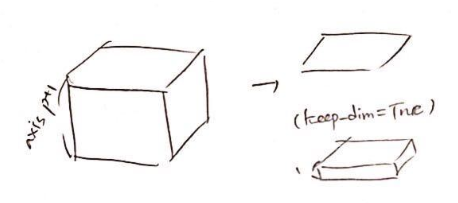
\includegraphics[height=8em]{resources/reduce.png}
}{
}{
  \begin{itemizec}
    \item $|y| = |input|$
  \end{itemizec}
}
\begin{align*}
  \frac
  {
    \begin{array}{l}
      \sigma \vdash E \Rar e, c
    \end{array}
  }
  {
    \sigma \vdash \op{threshold}{E, threshold, value, inplace=False} \Rar e, c
  }
\end{align*}

\subsection*{\texttt{torch.softmax}, \texttt{torch.nn.functional.softmax},
\texttt{torch.log\_softmax}, \texttt{torch.nn.functional.log\_softmax}}
\prepostc{torch.softmax(input, dim=None, \_stacklevel=3, dtype=None)
or torch.log\_softmax (same arguments)}{
  %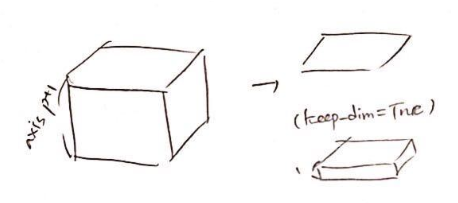
\includegraphics[height=8em]{resources/reduce.png}
}{
  \begin{itemizec}
    \item $-\op{rank}{|input|} \leq dim < \op{rank}{|input|}$
  \end{itemizec}
}{
  \begin{itemizec}
    \item $|y| = |input|$
  \end{itemizec}
}{
  \begin{itemizec}
    \item 원래 $dim = None$일 경우 last dimension이 기본값으로 들어갔지만,
    이제는 $dim = None$으로 쓰는 방식이 deprecated 되었다고 나와있음.
  \end{itemizec}
}
\begin{align*}
  \forall \mtt{ft} \in \{ \mtt{softmax}, \mtt{log\_softmax} \},\bigspace
  \frac
  {
    \begin{array}{l}
      \sigma \vdash E \Rar e, c \\
      c' = \{ (-\op{rank}{e} \leq dim < \op{rank}{e}) \}
    \end{array}
  }
  {
    \sigma \vdash \op{ft}{E, dim=None, \_stacklevel=3, dtype=None} \Rar e, c \cup c'
  }
\end{align*}

\subsection*{\texttt{torch.inverse}}
\prepostc{torch.inverse(input, out=None)}{
  %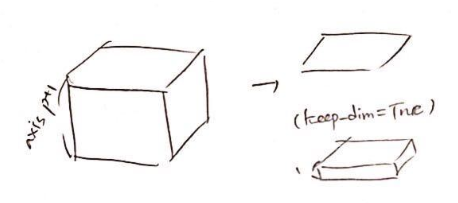
\includegraphics[height=8em]{resources/reduce.png}
}{
  \begin{itemizec}
    \item $|input| = (d_1, d_2, \dots, d_k)$
    \item $k \geq 2$
    \item $d_{k-1} = d_k$
  \end{itemizec}
}{
  \begin{itemizec}
    \item $|y| = |input|$
  \end{itemizec}
}{
  \begin{itemizec}
    \item 정사각행렬의 곱의 역원
    \item $out$-텐서 인자가 있는 함수
  \end{itemizec}
}
\begin{align*}
  \frac
  {
    \begin{array}{l}
      \sigma \vdash E \Rar e, c \\
      k = \op{rank}{e} \\
      c' = \{ (k \geq 2) \land (e[k-1] = e[k]) \}
    \end{array}
  }
  {
    \sigma \vdash \op{inverse}{E, out=None} \Rar e, c \cup c'
  }
\end{align*}

\subsection*{\texttt{torch.flip}}
\prepost{torch.flip(input, dims)}{
  %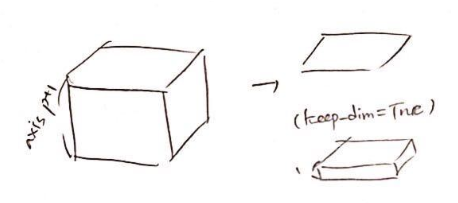
\includegraphics[height=8em]{resources/reduce.png}
}{
  \begin{itemizec}
    \item $|input| = (d_1, d_2, \dots, d_k)$
    \item $dims$ is a tuple or a list, and $\forall elt \in dims$, $-k \leq elt
    < k$.
  \end{itemizec}
}{
  \begin{itemizec}
    \item $|y| = |input|$
  \end{itemizec}
}
\begin{align*}
  \frac
  {
    \begin{array}{l}
      \sigma \vdash E \Rar e, c \\
      c' = \{ (\forall elt \in dims,\: -\op{rank}{e} \leq dim < \op{rank}{e}) \}
    \end{array}
  }
  {
    \sigma \vdash \op{flip}{E, dims} \Rar e, c \cup c'
  }
  \tag*{tuple 형태로 반환}
\end{align*}



\section*{Broadcasted Shape, Binary Operators}
All these builtin functions \texttt{torch.*} are used with
\texttt{torch.ft(input, other, out=None)} that output the same shapes of the
\texttt{input}s.
\begin{itemize}
  \item $\mtt{eq}, \mtt{le}, \mtt{lt}, \mtt{ge}, \mtt{gt}$
  \item $\mtt{mul}, \mtt{div}, \mtt{fmod}, \mtt{atan2}$
\end{itemize}
한 가지 독특한 성질은 $input$, $other$ 인자가 스칼라로 들어오면 $[\:]$-shape
텐서로 변환된 후 계산됩니다.
\begin{itemize}
  \item 즉, $\mtt{torch.mul}(1, 2)\mtt{.shape}$은 $[\:]$ 입니다.
\end{itemize}
\begin{align*}
  \frac
  {
    \begin{array}{l}
      \sigma \vdash E_1 \Rar e_1, c_1 \\
      \sigma \vdash E_2 \Rar e_2, c_2 \\
    \end{array}
  }
  {
    \sigma \vdash \op{ft}{E_1, E_2, out=None} \Rar broadcast(e_1, e_2),
      c_1 \cup c_2 \cup broadcastable(e_1, e_2)
  }
\end{align*}

The following builtin functions \texttt{torch.*} are slightly different.
\texttt{torch.ft(input, other, out=None, alpha=1)} that output the same shapes
of the \texttt{input}s. (Additional $alpha$ option!)
\begin{itemize}
  \item $\mtt{add}, \mtt{sub}$
  \begin{itemize}
    \item Calculates broadcasted $input \pm \alpha \cdot output$
  \end{itemize}
\end{itemize}
마찬가지로 $input$, $other$ 인자로 스칼라가 들어오면 $[\:]$-shape 텐서로 변환된
후 계산됩니다.
\begin{align*}
  \frac
  {
    \begin{array}{l}
      \sigma \vdash E_1 \Rar e_1, c_1 \\
      \sigma \vdash E_2 \Rar e_2, c_2 \\
    \end{array}
  }
  {
    \sigma \vdash \op{ft}{E_1, E_2, out=None, alpha=1} \Rar
      broadcast(e_1, e_2), c_1 \cup c_2 \cup broadcastable(e_1, e_2)
  }
\end{align*}

\subsection*{\texttt{torch.pow}}
\prepostc{torch.pow(input, exponent, out=None)}{}{
  \begin{itemizec}
    \item $[input$ or $exponent$ are scalar$]$
    \item[] or $broadcastable(|input|, |exponent|)$
  \end{itemizec}
}{
  \begin{itemizec}
    \item $broadcast(|input|, |exponent|)$
  \end{itemizec}
}{
  \begin{itemizec}
    \item elementwise binary operator라는 점에서 $\mtt{mul}$과 비슷하나, 인자
    이름(exponent)이 달라서 따로 뺐습니다. (\texttt{pow(a, exponent=b)}같은
    문제..)
    \item 마찬가지로 인자에 스칼라가 들어오면 $[\:]$-shape 텐서로 변환된 후
    계산됩니다.
    \item $out$ 인자가 있는 함수
  \end{itemizec}
}
\begin{align*}
  \frac
  {
    \begin{array}{l}
      \sigma \vdash E_1 \Rar e_1, c_1 \\
      \sigma \vdash E_2 \Rar e_2, c_2 \\
    \end{array}
  }
  {
    \sigma \vdash \op{pow}{E_1, E_2, out=None} \Rar broadcast(e_1, e_2),
      c_1 \cup c_2 \cup broadcastable(e_1, e_2)
  }
\end{align*}

\section*{Indexing}
\subsection*{\texttt{torch.Tensor.item}}
\prepostc{a.item()}{
  
\includegraphics[width=\linewidth]{resources/item.png}
}{
  \begin{itemizec}
    \item $|a| = ()$ or $|a| = (1, 1, 1, \dots, 1)$
  \end{itemizec}
}{
  \begin{itemizec}
    \item $|y| = e_n$
  \end{itemizec}
}{
  \begin{itemizec}
    \item Singular element tensor의 원소(스칼라 타입으로 반환)
  \end{itemizec}
}
\begin{align*}
  \frac
  {
    \begin{array}{l}
      \sigma \vdash E \Rar e, c \\
      k = \op{rank}{e} \\
      c' = \{ (\forall i = 1, 2, \dots, k,\: e[i] = 1) \}
    \end{array}
  }
  {
    \sigma \vdash E.\op{item}{} \Rar e_n, c \cup c'
  }
\end{align*}


\section*{Shape Polymorphism}
\subsection*{\texttt{torch.Tensor.view}}
\prepostc{a.view(n1, n2, ..., nl)}{
}{
  \begin{itemizec}
    \item $|\mtt{a}| = (d_1, d_2, \dots, d_k)$
    \item $reshapable((d_1, d_2, \dots, d_k), (n_1, n_2, \dots, n_l))$
  \end{itemizec}
}{
  \begin{itemizec}
    \item $(n_1, n_2, \dots, n_l)$ as tensor
  \end{itemizec}
}{
  \begin{itemizec}
    \item 단, $n_1, n_2, \dots, n_l$이 하나의 튜플로 입력이 들어올 수도 있음
  \end{itemizec}
}
\begin{align*}
  \frac
  {
    \begin{array}{l}
      \sigma \vdash \op{reshape}{E, n_1, n_2, \dots, n_l} \Rar e, c
    \end{array}
  }
  {
    \sigma \vdash E.\op{view}{n_1, n_2, \dots, n_l} \Rar e, c
  }
\end{align*}

\subsection*{\texttt{torch.Tensor.expand}}
\prepostc{a.expand(n1, n2, ..., nl)}{
  
\includegraphics[height=6em]{resources/expand.png}
}{
  \begin{itemizec}
    \item $|\mtt{a}| = (d_1, d_2, \dots, d_k)$
    \item $k \leq l$
    \item $\forall i = 1, 2, \dots, l-k$, $(n_i > 0)$
    \item $\forall i = l-k+1, l-k+2, \dots, l$, [($n_i = -1$) or (($n_i > 0$)
    and (($d_{i-(l-k)} = 1$) or ($d_{i-(l-k)} = n_i$)))]
  \end{itemizec}
}{
  \begin{itemizec}
    \item $(m_1, m_2, \dots, m_l)$ as tensor where
    \begin{itemize}
      \item $m_1 = n_1, m_2 = n_2, \cdots, m_{l-k} = n_{l-k}$
      \item $m_{l-k+i} = \ifs{(n_{l-k+i} = -1)}{d_i}{n_{l-k+i}}$ for the rests
    \end{itemize}
  \end{itemizec}
}{
  \begin{itemizec}
    \item 일방향 broadcast 함수; $(n_1, n_2, \dots, n_l)$ shape이 목표
    \item $n_i = -1$인 경우, 본래 크기만큼 그대로 유지
    \item 단, $n_1, n_2, \dots, n_l$이 하나의 튜플로 입력이 들어올 수도 있음
  \end{itemizec}
}
\begin{align*}
  \frac
  {
    \begin{array}{l}
      \sigma \vdash E \Rar e, c \\
      k = \op{rank}{e} \\
      m_1 = n_1, m_2 = n_2, \cdots , m_{l-k} = n_{l-k} \\
      \forall i \in \{1, 2, \dots, k\},\: m_{l-k+i}
        = \ifs{(n_{l-k+i} = -1)}{d_i}{n_{l-k+i}} \\
      c_{base} = \{ (k \leq l) \land (n_1 > 0) \land (n_2 > 0) \land \cdots
        \land (n_{l-k} > 0) \} \\
      c_{expandable} = \{ (\forall i \in \{1, 2, \dots, k\},\: (n_{l-k+i} = -1)
        \lor [(n_{l-k+i} > 0) \land ((d_{i}  = 1) \lor (d_{i} = n_{l-k+i}))]) \}
    \end{array}
  }
  {
    \sigma \vdash E.\op{expand}{n_1, n_2, \dots, n_l} \Rar
      (m_1, m_2, \dots, m_l), c \cup c_{base} \cup c_{expandable}
  }
\end{align*}

\subsection*{\texttt{torch.split}}
\prepostc{torch.split(tensor, split\_size\_or\_section, dim=0)}{
  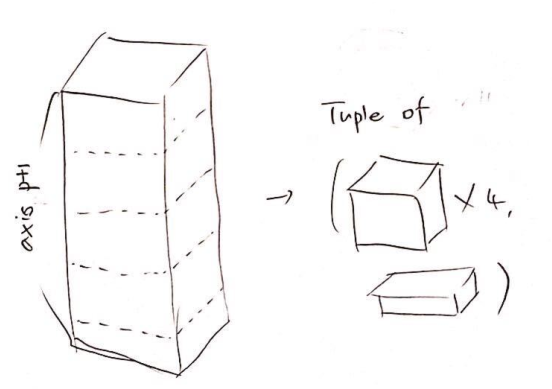
\includegraphics[height=14em]{resources/split1.png}
}{
  \begin{itemizec}
    \item $|tensor| = (d_1, d_2, \dots, d_k)$
    \item $k \geq 1$
    \item $0 \leq dim < k$
  \end{itemizec}
}{
  \begin{itemizec}
    \item 아래 proof tree와 같이 $dim+1$번째 axis가 최대
    $split\_size\_or\_section$개의 원소를 가지도록 $\lceil d_{dim+1} / \cdot \rceil$개
    튜플 형태로 반환
  \end{itemizec}
}{
  \begin{itemizec}
    \item Concat의 반대 역할 함수
    \item Divisible 여부 assert하지 않음
    \item 학습 및 테스트 데이터를 배치단위로 쪼개는 용도로 쓰일 것으로 추측
  \end{itemizec}
}
\begin{align*}
  \frac
  {
    \begin{array}{l}
      \sigma \vdash E \Rar e, c \\
      k = \op{rank}{e} \\
      e_1 = e\indr{1}{p} \conc (n) \conc e\indr{p+2}{k} \\
      e_2 = e\indr{1}{p} \conc (n) \conc e\indr{p+2}{k} \\
      \bigspace \cdots \\
      e_{l-1} = e\indr{1}{p} \conc (n) \conc e\indr{p+2}{k} \\
      e_l = e\indr{1}{p} \conc (n') \conc e\indr{p+2}{k} \bigspace
        \text{where $e \ind{p+1} = n(l-1) + n'$, $0 < n' \leq n$} \\
      c' = \{ (k \geq 1) \land (0 \leq p < k) \}
    \end{array}
  }
  {
    \sigma \vdash \op{split}{E, n, p=0} \Rar (e_1, e_2, \dots, e_l), c \cup c'
  }
  \tag*{$l$-원소 tuple 형태로 반환}
\end{align*}

\prepost{torch.split(input, [n1, n2, ..., nl], dim=0)}{
  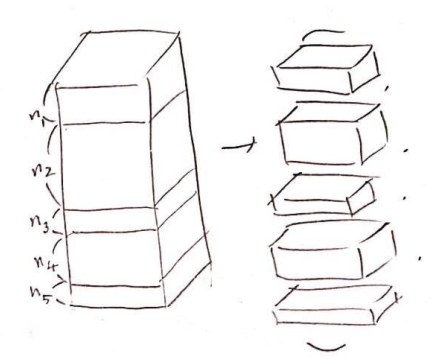
\includegraphics[height=14em]{resources/split2.png}
}{
  \begin{itemizec}
    \item $|input| = (d_1, d_2, \dots, d_k)$
    \item $k \geq 1$
    \item $0 \leq dim < k$
    \item $d_{dim+1} = n_1 + n_2 + \cdots + n_l$
  \end{itemizec}
}{
  \begin{itemizec}
    \item 아래 proof tree와 같이 $dim+1$번째 axis의 크기가 $n_1, n_2, \dots,
    n_l$인 $l$개의 텐서 튜플을 반환
    \item $n_i$의 합과 $d_{dim+1}$이 같은지 assert
  \end{itemizec}
}
\begin{align*}
  \frac
  {
    \begin{array}{l}
      \sigma \vdash E \Rar e, c \\
      k = \op{rank}{e} \\
      e_1 = e\indr{1}{p} \conc (n_1) \conc e\indr{p+2}{k} \\
      e_2 = e\indr{1}{p} \conc (n_2) \conc e\indr{p+2}{k} \\
      \bigspace \cdots \\
      e_l = e\indr{1}{p} \conc (n_l) \conc e\indr{p+2}{k} \\
      c' = \{ (k \geq 1) \land (0 \leq x < k) \land
        (e \ind{p+1} = n_1 + n_2 + \cdots + n_l) \}
    \end{array}
  }
  {
    \sigma \vdash \op{split}{E, \ind{n_1, n_2, \dots, n_l}, p=0}
      \Rar (e_1, e_2, \dots, e_l), c \cup c'
  }
  \tag*{$l$-원소 tuple 형태로 반환}
\end{align*}

\subsection*{\texttt{torch.chunk}}
\prepostc{torch.chunk(input, chunks, dim=0)}{
  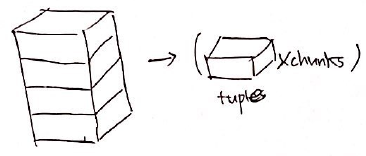
\includegraphics[height=9em]{resources/chunk.png}
}{
  \begin{itemizec}
    \item $|input| = (d_1, d_2, \dots, d_k)$
    \item $k \geq 1$
    \item $chunks > 0$
    \item $0 \leq dim < k$
  \end{itemizec}
}{
  \begin{itemizec}
    \item Proof tree와 같이 최소 $chunks$개로 $dim$ 축이 잘라진 텐서 튜플 반환
  \end{itemizec}
}{
  \begin{itemizec}
    \item \texttt{split}과 비슷하나 쪼개는 개수를 명시한다는 점이 다름
  \end{itemizec}
}
\begin{align*}
  \frac
  {
    \begin{array}{l}
      \sigma \vdash E \Rar e, c \\
      k = \op{rank}{e} \\
      d = \min\{ e[p+1], chunks \} \\
      n = \lceil e[p+1] / d \rceil \\
      e_1 = e\indr{1}{p} \conc (n) \conc e\indr{p+2}{k} \\
      e_2 = e\indr{1}{p} \conc (n) \conc e\indr{p+2}{k} \\
      \bigspace \cdots \\
      e_{l-1} = e\indr{1}{p} \conc (n) \conc e\indr{p+2}{k} \\
      e_l = e\indr{1}{p} \conc (n') \conc e\indr{p+2}{k} \bigspace
        \text{where $e \ind{p+1} = n(l-1) + n'$, $0 < n' \leq n$} \\
      c' = \{ (k \geq 1) \land (chunks > 0) \land (0 \leq p < k) \}
    \end{array}
  }
  {
    \sigma \vdash \op{chunk}{E, chunks, p=0} \Rar (e_1, e_2, \dots, e_l), c \cup c'
  }
  \tag*{$l$-원소 tuple 형태로 반환}
\end{align*}


\section*{Dynamic Operations (Cannot Predict Statically)}
\subsection*{\texttt{torch.nonzero}}
\prepostc{torch.nonzero(input, out=None, as\_tuple=False)}{
}{
}{
  \begin{itemizec}
    \item if $as\_tuple$, then $|y| = (countNonzeros(input), \op{rank}{|input|})$
    \item otherwise, then $|y|$ is $\op{rank}{|input|}$-tuple of tensors shaped
    $(countNonzeros(input))$
  \end{itemizec}
}{
  \begin{itemizec}
    \item $countNonzeros$는 주어진 텐서에서 $0$이 아닌 항의 개수를 구하는 것
    \item Nonzero 인덱스 번호들을 반환함.
    \item $out$-텐서 인자가 있는 함수
  \end{itemizec}
}
\begin{align*}
  \frac
  {
    \begin{array}{l}
      \sigma \vdash E_1 \Rar e_1, c_1 \\
      \sigma \vdash E_2 \Rar e_2, c_2 \\
    \end{array}
  }
  {
    \sigma \vdash \op{pow}{E_1, E_2, out=None} \Rar broadcast(e_1, e_2),
      c_1 \cup c_2 \cup broadcastable(e_1, e_2)
  }
\end{align*}
Example Codes:
\begin{Verbatim}[tabsize=4,xleftmargin=2em]
print(torch.nonzero(torch.tensor([[0, 1, 0], [0, 1, 1]])))
  # output: tensor([[0, 1], [1, 1], [1, 2]])
print(torch.nonzero(torch.tensor([[0, 1, 0], [0, 1, 1]]), as_tuple=True))
  # output: (tensor([0, 1, 1]), tensor([1, 1, 2]))
\end{Verbatim}

\end{document}
